\documentclass{article}

% Colors
\usepackage[dvipsnames]{xcolor}
% Float
\usepackage{float}
% Landscape
\usepackage{pdflscape}

% Tikz libraries
\usepackage{tikz}
\usepackage{tikz-3dplot}
\usetikzlibrary{arrows, calc}

% Values for plot
\tdplotsetmaincoords{60}{120}
\newcommand{\PointRho}{0.9}%
\newcommand{\PointTheta}{70}%
\newcommand{\PointPhi}{40}%


\begin{document}

\section{3D Plot}

\begin{tikzpicture}
    [scale=8,
        tdplot_main_coords,
        axis/.style={->,blue,thick},
        vector/.style={-stealth,red,very thick},
        vector guide/.style={dashed,red,thick}]

    % Tikz coordinate (x, y, z)
    \coordinate (Origin) at (0,0,0);
    % Tikz-3dplot spherical coordinate (rho, theta, phi)
    \tdplotsetcoord{Point}{\PointRho}{\PointTheta}{\PointPhi}

    % Axes
    \draw[axis, black] (0,0,0) -- (1,0,0) node[anchor=north east]{\(x\)};
    \draw[axis, black] (0,0,0) -- (0,1,0) node[anchor=north west]{\(y\)};
    \draw[axis, black] (0,0,0) -- (0,0,1) node[anchor=south]{\(z\)};

    % Vector from Origin
    \draw[vector] (Origin) -- (Point);

    % Guides to vector components
    % Point -> Pointx, Pointy, Pointz, Pointxy, Pointyz, Pointxz
    % Guide on plane xy from Origin
    \draw[vector guide] (Origin) -- (Pointxy);
    % Guide from plane xy to Point
    \draw[vector guide] (Pointxy) -- (Point);

    % Find (x,y,z) from (rho, theta, phi)
    \pgfmathsetmacro{\PointxCoord}{\PointRho * sin(\PointPhi) * cos(\PointTheta)}
    \pgfmathsetmacro{\PointyCoord}{\PointRho * sin(\PointPhi) * sin(\PointTheta)}
    \pgfmathsetmacro{\PointzCoord}{\PointRho * cos(\PointPhi)}

    \draw[vector guide, purple] (Pointxy) -- (Pointx) node [above left]  {\PointxCoord};
    \draw[vector guide, purple] (Pointxy) -- (Pointy) node [above right] {\PointyCoord};

    \draw[vector guide, olive] (Point) -- (Pointxz) node [left]  {\PointxCoord};
    \draw[vector guide, olive] (Point) -- (Pointyz) node [right] {\PointyCoord};

    \draw[vector guide, magenta] (Pointyz) -- (Pointz) node [left] {\PointzCoord};
\end{tikzpicture}


\section{A box ?}

\begin{tikzpicture}
    [scale=8,
        tdplot_main_coords,
        axis/.style={->,blue,thick},
        vector/.style={-stealth,red,very thick},
        vector guide/.style={dashed,red,very thick}]

    % Tikz coordinate (x, y, z)
    \coordinate (Origin) at (0,0,0);
    % Tikz-3dplot spherical coordinate (rho, theta, phi)
    \tdplotsetcoord{Point}{\PointRho}{\PointTheta}{\PointPhi}

    % Axes
    \draw[axis, black] (0,0,0) -- (1,0,0) node[anchor=north east]{\(x\)};
    \draw[axis, black] (0,0,0) -- (0,1,0) node[anchor=north west]{\(y\)};
    \draw[axis, black] (0,0,0) -- (0,0,1) node[anchor=south]{\(z\)};

    % Draw box
    % Axis parallel to z
    \draw[vector guide, Red] (Origin) -- (Pointz);
    \draw[vector guide, Red] (Pointx) -- (Pointxz);
    \draw[vector guide, Red] (Pointy) -- (Pointyz);
    \draw[vector guide, Red] (Pointxy) -- (Point);

    % Axis parallel to x
    \draw[vector guide, Blue] (Origin) -- (Pointx);
    \draw[vector guide, Blue] (Pointy) -- (Pointxy);
    \draw[vector guide, Blue] (Pointz) -- (Pointxz);
    \draw[vector guide, Blue] (Pointyz) -- (Point);

    % Axis parallel to y
    \draw[vector guide, Green] (Origin) -- (Pointy);
    \draw[vector guide, Green] (Pointx) -- (Pointxy);
    \draw[vector guide, Green] (Pointz) -- (Pointyz);
    \draw[vector guide, Green] (Pointxz) -- (Point);

\end{tikzpicture}

\begin{landscape}
    % Page numbering
    \thispagestyle{empty}

    \section{Computer Vision Processes}

    These figures were made to illustrate two computer vision processes. Theses processes can be used in robotic systems.

    \begin{center}
        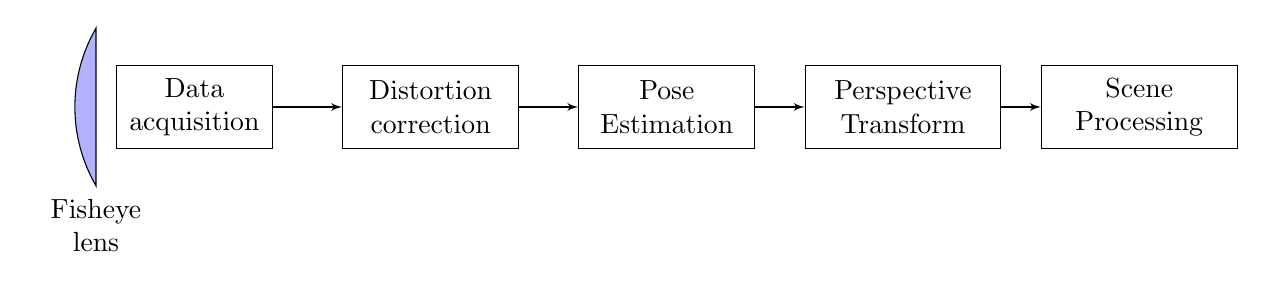
\begin{tikzpicture}[auto,scale=2, node distance=3cm,>=latex', text width=1.5cm, align=center,block/.style = {draw, fill=white, rectangle, minimum height=3em, minimum width=3em}]
            \pgfmathsetmacro{\lensRadius}{2}
            \pgfmathsetmacro{\lensHeight}{1}
            \pgfmathsetmacro{\startAngle}{asin(\lensHeight/\lensRadius)}

            % Lens
            \coordinate (lens) at (0,0);
            \draw [fill=blue!30, scale=0.5]  ($ (lens) + (0, \lensHeight)$)
            arc[start angle=180-\startAngle,delta angle=2*\startAngle,radius=\lensRadius] -- cycle;
            \node [below of=lens, node distance=1.5cm, text width=1.5cm] (lensIndic) {Fisheye lens};

            \node [block, right of=lens, node distance=1.25cm, text width=1.75cm] (camera) {Data acquisition};
            \node [block, right of=camera, node distance=3cm, text width=2cm] (distortion) {Distortion correction};
            \node [block, right of=distortion, node distance=3cm, text width=2cm] (pose) {Pose Estimation};
            \node [block, right of=pose, node distance=3cm, text width=2.25cm] (perspective) {Perspective Transform};
            \node [block, right of=perspective, node distance=3cm, text width=2.25cm] (scene) {Scene Processing};

            \draw [->] (camera) -- node {} (distortion);
            \draw [->] (distortion) -- node {} (pose);
            \draw [->] (pose) -- node {} (perspective);
            \draw [->] (perspective) -- node {} (scene);
        \end{tikzpicture}
    \end{center}

    \vfill

    \begin{center}
        \begin{tikzpicture}[auto, scale=2, node distance=3cm,>=latex', text width=1.5cm, align=center, block/.style = {draw, fill=white, rectangle, minimum height=3em, minimum width=3em}]
            \pgfmathsetmacro{\lensRadius}{2}
            \pgfmathsetmacro{\lensHeight}{1}
            \pgfmathsetmacro{\startAngle}{asin(\lensHeight/\lensRadius)}

            % Lens
            \coordinate (lens) at (0,0);
            \draw [fill=blue!30, scale=0.5]  ($ (lens) + (0, \lensHeight)$)
            arc[start angle=180-\startAngle,delta angle=2*\startAngle,radius=\lensRadius] -- cycle;
            \node [below of=lens, node distance=1.5cm, text width=1.5cm] (lensIndic) {Lens};

            \node [block, right of=lens, node distance=1.25cm, text width=1.75cm] (camera) {Data acquisition};
            \node [block, right of=camera, node distance=3cm, text width=2cm] (roi) {Region of image};
            \node [block, right of=roi, node distance=3cm, text width=2cm] (thresholding) {Thresholding};
            \node [block, right of=thresholding, node distance=3cm, text width=2.25cm] (binarisation) {Processing};
            \node [block, right of=perspective, node distance=3cm, text width=2.25cm] (decision) {Decision making};

            \draw [->] (camera) -- node {} (roi);
            \draw [->] (roi) -- node {} (thresholding);
            \draw [->] (thresholding) -- node {} (binarisation);
            \draw [->] (binarisation) -- node {} (decision);
        \end{tikzpicture}
    \end{center}
\end{landscape}

\end{document}